%%%%%%%%%%%%%%%%%%%%%%%
%
% © Pierre-Louis Gstalter
% 02/16/2022
%
%%%%%%%%%%%%%%%%%%%%%%%
\documentclass{article}
\usepackage[french]{babel}
\usepackage[left=1cm, right=1cm, top=1.5cm, bottom=1cm]{geometry}
\usepackage{multicol}
\usepackage{color}
\usepackage{graphicx}
\usepackage{hyperref}
\setlength{\columnseprule}{0pt}
\def\columnseprulecolor{\color{blue}}
\pagestyle{empty}

\begin{document}
\begin{multicols}{3}

Paris

pierre-louis.gstalter@minesparis.psl.eu

\texttt{+33647437563}

plgstalter.org

github.com/plgstalter

\columnbreak

	\hfill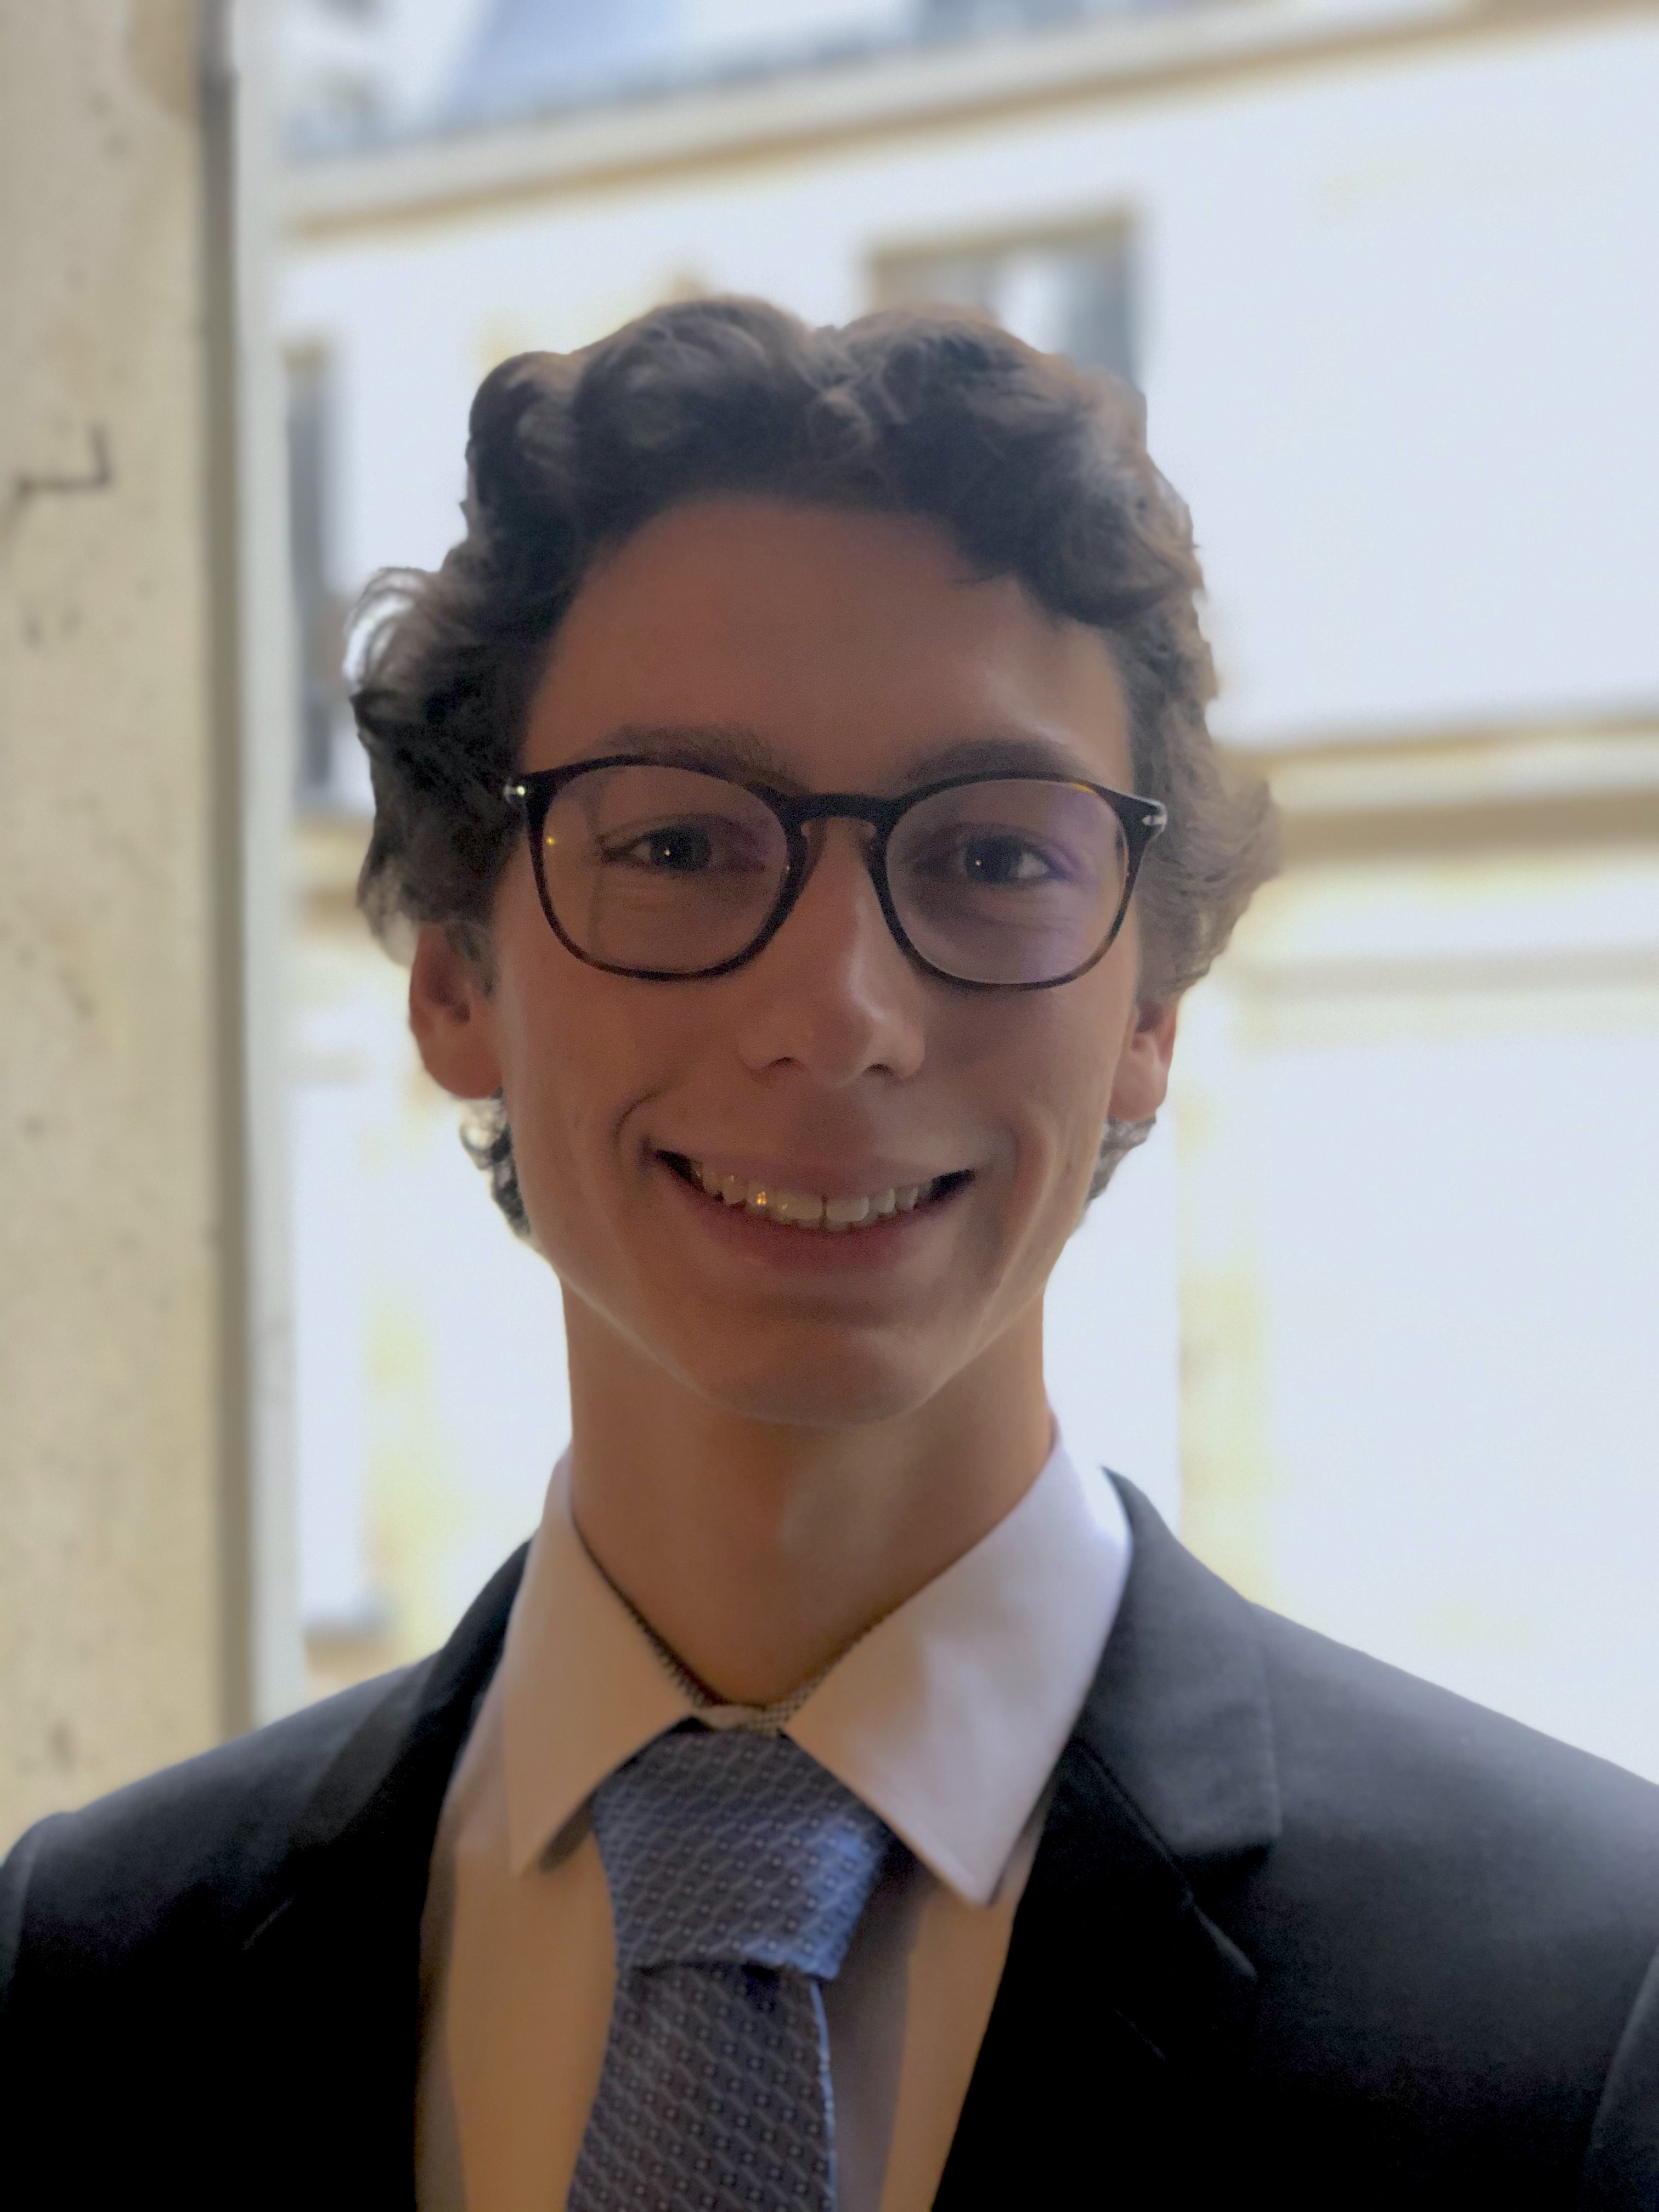
\includegraphics[width=2.6cm]{photo.jpeg}

\columnbreak

{\color{blue} \section*{Pierre-Louis Gstalter}}

\noindent Élève de deuxième année aux Mines de Paris en cursus Ingénieur Civil, je suis passionné de mathématiques et d'informatiques et suis à la recherche d'un stage dans le domaine de la finance.
\end{multicols}

\setlength{\columnsep}{2cm}
\setlength{\columnseprule}{1.5pt}
\begin{multicols}{2}
	{\color{blue} \subsection*{Formation}}

		\noindent\texttt{2020-2024} \textbf{Mines de Paris}

		\textbf{Mathématiques : } probabilités, optimisation, 

		statistiques, algèbre

		\textbf{Informatique : } analyse de données, programmation 

		orientée objet

\hfill

		\noindent\texttt{2021-2022} \textbf{Università degli Studi di Milano}

		Échange Erasmus+, cours en anglais et italien

		Mathématiques financières, algorithmes heuristiques, 

		optimisation combinatoire

\hfill

		\noindent\texttt{2018-2020} \textbf{Lycée Henri IV}
		
		Classes Préparatoires aux Grandes Écoles MPSI-MP

\hfill

		\noindent\texttt{2018} \textbf{Gymnase Jean Sturm}

		Baccalauréat scientifique. Mention très bien, 18.32/20

\hfill

	{\color{blue} \subsection*{Expériences Professionnelles}}

		\noindent\texttt{02/2022-?} \textbf{Colleur de mathématiques}

		Lycée Henri IV, Paris


		\noindent\texttt{09/2020-?} \textbf{Professeur particulier}

		mathématiques et physique, niveau lycée à CPGE, à 

		domicile ou en ligne

\hfill
	
		\noindent\texttt{05/2021} \textbf{Vendeur, stage exécutant}

		Endurance Shop Strasbourg

\hfill

		\noindent\texttt{2018-2019} \textbf{Moniteur de canoë-kayak}

		ASCPA Strasbourg

\hfill

{\color{blue} \subsection*{Expériences Informatiques}}

		\begin{itemize}
			\item[\texttt{2022}]
				Implémentation de l'algorithme de Dijkstra en C++, calcul empirique de complexité sur différentes structures de données.
	
			\hfill

			\item[\texttt{2021}]
				Travail sur des bases de données à propos d'éoliennes en Python (pandas, sklearn, matplotlib). Avec \textbf{Engie Digital}.

			\hfill

			\item[$\circ$]
				Création, hébergement et maintenance de mon site personnel : plgstalter.org 
		
			\hfill

			\item[$\circ$]
				Réparation de matériel informatique: remplacement de composants et réparation logicielle

			\hfill

			\item[$\circ$]
				Membre d'Anonymines, l'association informatique des Mines de Paris. Organisation d'événements avec des entreprises.
		\end{itemize}

\columnbreak
	{\color{blue} \subsection*{Langues}}

		\begin{itemize}
			\item[$\circ$]
			\textbf{Français : } langue maternelle
		\item[$\circ$]

			\textbf{Anglais : } bilingue
		\item[$\circ$]

			\textbf{Allemand :} niveau B2
		\item[$\circ$]

			\textbf{Italien :} niveau B2
		\end{itemize}

	{\color{blue} \subsection*{Compétences Informatiques}}

		\noindent\textbf{Langages de programmation}

		avancé : Python, C++, bash
				
		bases : javascript, MySQL, PHP, Swift, MATLAB

\hfill

		\noindent\textbf{Edition de texte}

		html, CSS, LaTeX, R Markdown

\hfill

		\noindent\textbf{Logiciels}

		vim, git, GIMP, bash, VS Code, Xcode

\hfill

		\noindent\textbf{Systèmes d'exploitation}

		Mac OS, Linux

\hfill

{\color{blue} \subsection*{Diplômes}}

		\noindent\texttt{2022} \textbf{Introduction to Market Microstructure}

		Institut Louis Bachelier, MOOC sur la microstructure de marchés financiers

\hfill

		\noindent\texttt{2018} \textbf{Cambridge First Assessment}

		Obtenu avec le grade C1 (182/190)

\hfill

		\noindent\texttt{2017-2018} \textbf{AMFPC}

		Diplôme d'encadrement de la pratique du canoë-kayak

\hfill

{\color{blue} \subsection*{Sport}\label{sport}}

		\noindent\textbf{Course à pied}

		$\sim$100km par semaine, 1h17 au semi-marathon

\hfill

		\noindent\textbf{Kayak}

		9 ans de pratique, compétitions de niveau national et 

		encadrement

\hfill

{\color{blue} \subsection*{Loisirs}}

		\noindent\textbf{Cinéma}

		membre du \textit{Club Ciné} des Mines de Paris

\hfill

		\noindent\textbf{Finance}

		Achat et revente d'actions du CAC 40 depuis avril 2020

\end{multicols}
\end{document}

%%%%%%%%%%%%%%
%
% last updated: 02/17/2022
%
%%%%%%%%%%%%%%
